\chapter{计算模型}
\label{chapter:model}

\section{神经元模型}
\label{section:model:neuron-model}

常见的神经元模型包括 Hodgkin-Huxley 模型和 Integrate-and-Fire 模型。
前者可以模拟细胞膜上各种离子通道,通过调整参数,可以模拟出大量的特性。
后者不模拟离子通道的细节,只模拟细胞膜电位的变化,计算更高效。
介于两只之间的有 Izhikevich 模型,模型的部分参数失去了直观的物理意义,但通过调整参数,可以模拟出很多典型的神经元发放特性,同时计算也比 Hodgkin-Huxley 模型高效很多 \cite{Izhikevich2003,Izhikevich2004}。

\subsection{Izhikevich 模型}
Izhikevich 模型的动力学方程如下
\begin{align}
C \frac{\dd{v}}{\dd{t}} &= k \left( v-v_\text{r} \right) \left( v-v_\text{t} \right) - u + I \label{equation:izhikevich-membrane} \\
\frac{\dd{u}}{\dd{t}} &= a \left\{ b \left( v-v_\text{r} \right) - u \right\} \label{equation:izhikevich-recovery-current} \\
\text{当} v \geq v_{\text{peak}} \text{时,} & v \leftarrow c, u \leftarrow u + d \label{equation:izhikevich-spike}
\end{align}
其中 $v$ 是细胞膜电位, $u$ 是恢复电流, $C$ 是细胞膜电容, $v_\text{r}$ 是细胞膜静息电位, $v_\text{t}$ 是细胞膜自主发放电位。
$a$, $b$, $c$, $d$,和 $k$是其他参数, $I$ 是外部输入的电流。

在模拟 Fast-Spiking 神经元时,对模型中的式\ref{equation:izhikevich-recovery-current}进行一些改动,
\begin{align}
\frac{\dd{u}}{\dd{t}} &= 0.2 \left\{ U\left( v \right) - u \right\} \label{equation:izhikevich-fast-spiking} \\
U\left( v \right) &= \begin{cases} 0, &\mbox{当} v < v_\text{b} \mbox{时} \\ 0.025, &\mbox{当} v \geq v_\text{b} \mbox{时} \end{cases}
\end{align}
各项参数为
\begin{align*}
C &= 20\ \text{pF}, \\
k &= 1\ \text{pA} \cdot \text{mV$^{-2}$}, \\
v_\text{r} &= -55\ \text{mV}, \\
v_\text{t} &= -40\ \text{mV}, \\
v_\text{b} &= -55\ \text{mV}, \\
v_\text{peak} &= 25\ \text{mV}, \\
c &= -45\ \text{mV}.
\end{align*}

\section{突触模型}
\label{section:model:synapse-model}
流行的描述突触动态性的模型有 Misha Tsodyks 和 Henry Markram 提出的短时程突触可塑性(Short-Term Synaptic Plasticity)模型\cite{Markram1996,Tsodyks1997}。
最新版本的模型如下\cite{Tsodyks2013}

\begin{align}
\frac{\dd{u\left(t\right)}}{\dd{t}} &=  -\frac{u\left(t\right)}{\tau_f}+U\left[1-u\left(t\right)\right]\sum_m \delta\left(t-t_m\right), \label{equation:stp-facilitation} \\
\frac{\dd{x\left(t\right)}}{\dd{t}} &=
\frac{X_F-x\left(t\right)}{\tau_d} - q(t),
\label{equation:stp-depression} \\
q(t) & = u\left(t_+\right)x\left(t_-\right) \sum_m \delta\left(t-t_m\right),
\label{equation:stp-release}
\end{align}
其中 $u$ 代表细胞膜内钙离子残余造成的递质释放概率提升, $x$ 代表剩余的可释放递质的量, $q$ 代表递质的释放速率。 
$X_F$ 是静息状态下突触的可释放递质的总量。 
$\tau_f$, $U$, $\tau_d$ 是其他参数。不同类型的神经元有不同的参数 \cite{Silberberg2005}。

释放出的递质 $q$ 与突触后神经元上的递质接收器结合,产生突触后神经元细胞膜电流等一系列变化。
这部分也可以用模型描述\cite{Destexhe1994}。
\begin{align}
I_\text{syn}(t) &= g(t)\left(v(t) - E_\text{syn}\right), \label{equation:synaptic-current-general} \\
\frac{\dd{g(t)}}{\dd{t}} &= -\frac{g(t)}{\tau_\text{syn}} + wq(t - t_\text{delay}), \label{equation:receptor-conductance-general}
\end{align}
其中 $v$ 是突触后细胞的膜电位, $g$ 是离子通道的电导, $E_\text{syn}$ 是离子的反转电位, $w$ 是突触权重, $t_\text{delay}$ 是由于递质传递造成的延迟。

\subsection{非同步递质释放模型}
\label{section:model:asynchronous-release}
基于短时程突触可塑性模型,我们提出非同步递质释放模型,在原模型的基础上,增加非同步释放机制。
基于囊泡上存在两类不同特性的钙离子感受器,我们将式\ref{equation:stp-facilitation}分成两个形式一致,但具有不同参数的过程。
\begin{align}
\frac{\dd{u_\text{sr}\left(t\right)}}{\dd{t}} &= -\frac{u_\text{sr}\left(t\right)}{\tau_\text{sr}}+U_\text{sr}\left[1-u_\text{sr}\left(t\right)\right]\sum_m \delta\left(t-t_m\right), \label{equation:sr-facilitation} \\
\frac{\dd{u_\text{ar}\left(t\right)}}{\dd{t}} &= -\frac{u_\text{ar}\left(t\right)}{\tau_\text{ar}}+U_\text{ar}\left[1-u_\text{ar}\left(t\right)\right]\sum_m \delta\left(t-t_m\right), \label{equation:ar-facilitation}
\end{align}
其中 $u_\text{sr}$ 和 $u_\text{ar}$ 是由于钙离子参与造成的造成的同步释放与非同步释放的不同的激活程度。
$U_\text{sr}$ 和 $U_\text{ar}$ 控制每个动作电位之后同步释放与非同步释放激活程度的提升大小。
$\tau_\text{sr}$ 和 $\tau_\text{ar}$ 控制钙离子感受器与钙离子分离造成同步释放与非同步释放激活程度下降的速度。

由于有实验支持同步释放和非同步释放竞争同一个递质资源池\cite{Otsu2004,Wen2010},所以使用单个变量 $x$ 来代表剩余的递质量,依旧沿用式\ref{equation:stp-depression}。

沿用原模型里的描述,只有动作电位到达后的短暂时刻有同步释放,同步释放的释放率为
\begin{equation}
q_\text{sr}(t) = u_\text{sr}(t_+)x(t_-)\sum_m \delta(t-t_m). \label{equation:sr-release}
\end{equation}

非同步释放则是高度随机的事件。
随机性使用二项过程模拟 \cite{DELCASTILLO1954}。
随机变量 $n$ 服从二项分布, $n\sim{\cal{B}}\left(N,p\right)$, 则它的概率分布函数为 $P(n=k|N,p) = \binom{N}{k} p^k (1-p)^{N-k}$, 其中 $k\in\{0,\ldots,N\}$, 且 $p$ 是单个事件发生的概率。

假设每个囊泡所含递质量相同,记为释放量子 $x_0$ ,那么在时刻 $t$ 剩余的可以释放的囊泡数量则有 $\sim \left\lfloor x(t)/x_0 \right\rfloor$ ,其中 $\lfloor \cdot \rfloor$ 表示取向下取整函数,取不大于自变量的最大整数。
在一个小的时间段 $[t,t+\dd{t})$ 内,单个囊泡由于非同步释放的钙离子感受器激活导致释放的释放概率为 $u_\text{ar}(t)\dd{t}$ 。
那么,非同步释放事件发生的数量 $n(t)$ 服从二项分布 ${\cal{B}}\left(\left\lfloor x(t)/x_0\right\rfloor,u_\text{ar}(t)\dd{t}\right)$。
因此,在时间段 $[t,t+\dd{t})$ 内释放的递质量为
\begin{equation}
  q_\text{ar}(t)\dd{t} = x_0 n(t), \label{equation:ar-release}
\end{equation}
其中 $n(t)$ 是上文定义的二项随机数。

在计算某段时间内同步释放与非同步释放的总和时,需要注意有些囊泡上可能同步释放和非同步释放的钙离子感受器同时激活,这部分递质量不应该被重复累加。
当时间段 $[t,t+\dd{t})$ 内发生了同步释放时,即有动作电位在这一时间段内到达,这部分同步释放和非同步释放的钙离子感受器同时激活导致的递质释放量为
\begin{equation}
q_\text{s\&a}(t)\dd{t} = q_\text{ar}(t)\dd{t}u_\text{sr}(t_+).
\end{equation}
如果在这一时间段内没有动作电位到达,那么 $q_\text{s\&a}(t) = 0$ 。

综上, $t$ 时刻总的递质释放率为
\begin{equation}
q(t) = q_\text{ar}(t) +q_\text{sr}(t) - q_\text{s\&a}(t). \label{equation:total-release}
\end{equation}

式\ref{equation:sr-facilitation},\ref{equation:ar-facilitation},\ref{equation:stp-depression},和\ref{equation:total-release}描述了扩展后模型的突触动力学。图\ref{figure:model-diagram}为模型的示意图。

\begin{figure}[h]
\centering
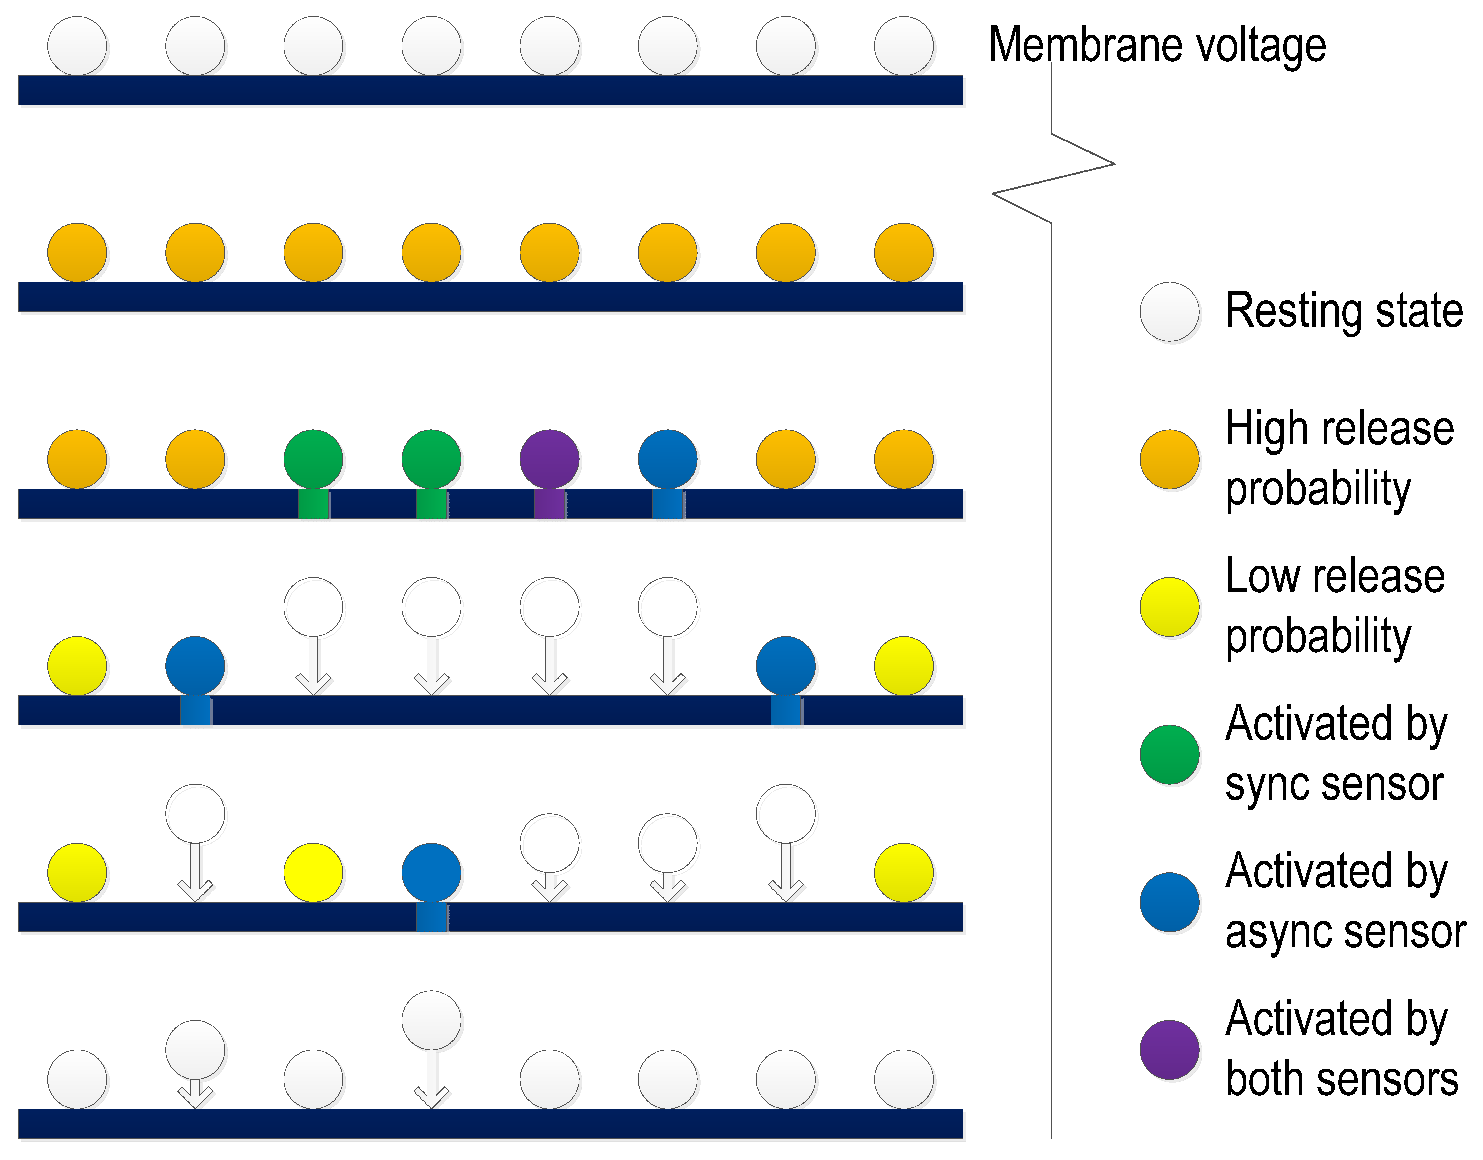
\includegraphics[scale=0.5]{model-diagram.eps}
\caption{同步释放与非同步释放突触模型示意图。描述突触在从静息状态,到遇到动作电位,再回到静息状态的时间过程中各个阶段的变化。
第一行:突触处于静息状态,囊泡停泊在细胞膜上的活动区,准备释放,与囊泡上的钙离子感受器结合的钙离子较少,囊泡激活程度极低(用白色表示)。
第二行:一个动作电位过后,钙离子大量进入细胞内,与囊泡上的钙离子感受器结合,此时囊泡有较高的释放概率(用橙色表示)。
第三行:紧接着动作电位结束,一些囊泡被钙离子感受器激活(标记为绿色,蓝色,和紫色),开始与细胞膜融合并释放递质。这些囊泡有的是被同步释放的钙离子感受器激活(用绿色表示),有的是被非同步释放的钙离子感受器激活(用蓝色表示),还有的是两种钙离子感受器同时激活(用紫色表示)。
第四行:囊泡释放后细胞会新合成一些来补充到活动区(用箭头表示),在完成停泊上细胞膜之前这些囊泡无法释放。由于细胞内的钙离子清除机制,钙离子浓度会下降,剩余的可以释放的囊泡的释放概率降低。但仍有一些可以进行非同步释放(用蓝色表示)。
第五行:随着囊泡释放概率的降低,被非同步释放的钙离子感受器激活的囊泡越来越少。
第六行:钙离子浓度回到静息状态,等待下一个动作电位。}
\label{figure:model-diagram}
\end{figure}

\section{网络模型}
\label{section:model:network-model}
网络模型使用 Izhikevich 神经元模型,与带有非同步释放特性的突触模型结合组成抑制性 Fast-Spiking 神经元网络。
总共取 $n$ 个神经元,神经元之间随即链接,链接概率为 $p$。

\section{简化模型}
\label{section:model:simplified-model}
